\documentclass[aspectratio=169,11pt]{beamer}

% =============================================================================
% 1. PRESENTATION METADATA CONFIGURATION
% =============================================================================
\newcommand{\reviewBanner}{EVALUATION II}
\newcommand{\presentationTitle}{SPECTRA: AN ADVANCED SIDE-CHANNEL HARDWARE TROJAN DETECTION\\FRAMEWORK VIA ADAPTIVE HARMONIC ENERGY AND MULTIMODAL METRIC FUSION}
\newcommand{\presentationSubtitle}{Phase 2: Advanced Novelty, Comprehensive Stress-Testing \& Publication Readiness}
\newcommand{\academicYear}{AY 2026--2027}

% Team Member Credentials
\newcommand{\memberOneRoll}{BL.EN.U4ECE23205}
\newcommand{\memberOneName}{Chandan Sai Pavan Padala}
\newcommand{\memberTwoRoll}{BL.EN.U4ECE23226}
\newcommand{\memberTwoName}{M Madhumitha}
\newcommand{\memberThreeRoll}{BL.EN.U4ECE23227}
\newcommand{\memberThreeName}{M V Sri Harsha}

% Project Supervision
\newcommand{\guideName}{Dr. Paramasivam C.}

% Footer Branding & University Credentials
\newcommand{\footerTeamName}{Team SPECTRA}
\newcommand{\departmentName}{Department of Electronics and Communication Engineering}
\newcommand{\campusName}{Amrita School of Engineering, Bengaluru \quad$\bullet$\quad Amrita Vishwa Vidyapeetham}

% Total Slides for Footer Counter
\providecommand{\totalSlideCount}{15}

% Logo Asset Selection (color, dark, or white)
\newcommand{\logoAsset}{Amrita-vishwa-vidyapeetham-white-logo.png}

% Background Gradient Toggle
\def\useGradientBackground{1}

% =============================================================================
% 2. THEME & PACKAGE INCLUSION
% =============================================================================
\usepackage{beamer_amrita_theme}
\usetikzlibrary{arrows.meta,positioning,shapes,calc,fit,backgrounds}
\usepackage[none]{hyphenat}
\hyphenpenalty=10000
\exhyphenpenalty=10000
\binoppenalty=10000
\relpenalty=10000
\tolerance=10000
\emergencystretch=3em
\righthyphenmin=62
\lefthyphenmin=62

% Background Canvas Setup (Full-bleed seamless coverage)
\ifdefined\useGradientBackground
  \setbeamercolor{background canvas}{bg=}
  \setbeamertemplate{background}{}
  \setbeamertemplate{background canvas}{%
    \vbox to \paperheight{\vss
      \hbox to \paperwidth{\hss
        
\includegraphics[width=\dimexpr\paperwidth+4mm\relax, height=\dimexpr\paperheight+4mm\relax, keepaspectratio=false]{background-gradient.png}%
      \hss}%
    \vss}%
  }
\else
  \setbeamercolor{background canvas}{bg=canvasBg}
  \setbeamertemplate{background}{}
\fi

% =============================================================================
% DOCUMENT CONTENT (15 SLIDES: COMPREHENSIVE NOVELTY & STRESS TESTING FOR EVAL 2)
% =============================================================================
\begin{document}

% -----------------------------------------------------------------------------
% SLIDE 1: MASTER TITLE SLIDE
% -----------------------------------------------------------------------------
\begin{frame}[t]
  \vspace*{-0.35cm}
  \noindent
  \hfill
  \begin{minipage}[c]{0.5\textwidth}
    \raggedleft
    \includegraphics[height=0.80cm, keepaspectratio]{\logoAsset}%
    \hspace*{-0.80cm}%
  \end{minipage}%

  \vspace{0.06cm}
  \begin{glasscard}[opacityback=0.18, arc=3.5mm, top=5pt, bottom=5pt, left=8pt, right=8pt]
    \begin{center}
      \tikz\node[draw=accentDark, line width=1.1pt, rounded corners=4pt, fill=white, fill opacity=0.65, text opacity=1, inner xsep=14pt, inner ysep=3.5pt]{%
        {\fontsize{11pt}{13pt}\selectfont\bfseries\color{accentDark} \reviewBanner}%
      };
      \vspace{0.10cm}

      {\fontsize{10.2pt}{13.5pt}\selectfont\bfseries\color{textPrimary} \presentationTitle}
      \vspace{0.10cm}

      \noindent
      {\color{accentDark}\rule[3pt]{0.03\linewidth}{1.1pt}} \quad
      {\fontsize{8.5pt}{11.0pt}\selectfont\bfseries\color{textPrimary} \presentationSubtitle} \quad
      {\color{accentDark}\rule[3pt]{0.03\linewidth}{1.1pt}}
      \vspace{0.06cm}

      {\fontsize{7.5pt}{9.5pt}\selectfont\color{black!75} Evaluated Against Reference Paper: Chunhua He et al., \textit{IEEE Internet of Things Journal}, Vol.\ 11, No.\ 8, April 2024}
    \end{center}
  \end{glasscard}

  \vspace{0.06cm}
  \begin{columns}[T]
    \begin{column}{0.49\textwidth}
      \begin{glasscard}[top=3.5pt, bottom=3.5pt, left=6pt, right=6pt]
        {\color{accentDark}\rule[-1pt]{2.5pt}{9pt}}\hspace{5pt}%
        {\fontsize{9.5pt}{11.5pt}\selectfont\bfseries\color{textPrimary} TEAM MEMBERS:}\\[2.5pt]
        {\fontsize{8.5pt}{11.0pt}\selectfont\color{textPrimary}
        \memberOneRoll\ --- \memberOneName\\
        \memberTwoRoll\ --- \memberTwoName\\
        \memberThreeRoll\ --- \memberThreeName}
      \end{glasscard}
    \end{column}
    \begin{column}{0.49\textwidth}
      \begin{glasscard}[top=3.5pt, bottom=3.5pt, left=6pt, right=6pt]
        {\color{accentDark}\rule[-1pt]{2.5pt}{9pt}}\hspace{5pt}%
        {\fontsize{9.5pt}{11.5pt}\selectfont\bfseries\color{textPrimary} PROJECT SUPERVISION:}\\[2.5pt]
        {\fontsize{8.5pt}{11.0pt}\selectfont\color{textPrimary}
        \textbf{\color{textPrimary}Course Instructor \& Guide:}\hspace{0.5em} \color{textPrimary}\guideName\\
        {\fontsize{7.8pt}{9.8pt}\selectfont\color{black!70} 23ECE341 --- Hardware Security and Trust}\\[1.5pt]
        {\fontsize{7.8pt}{9.8pt}\selectfont\color{black!70} Amrita School of Engineering, Bengaluru}}
      \end{glasscard}
    \end{column}
  \end{columns}
\end{frame}

% -----------------------------------------------------------------------------
% SLIDE 2: EXECUTIVE CONTEXT — FROM BASE PAPER TO SPECTRA
% -----------------------------------------------------------------------------
\begin{frame}[t]
  \slideheader{EXECUTIVE CONTEXT: FROM BASE PAPER TO SPECTRA}
  \vspace*{-0.18cm}

  \begin{columns}[T, onlytextwidth]
    \begin{column}{0.485\textwidth}
      \begin{glassbox}[top=2pt, bottom=2pt, left=6pt, right=6pt, title={Evaluation 1 Accomplishments (Recap)}]{}
        \begin{itemize}\setlength{\itemsep}{1.2pt}
          \item \textbf{100\% Faithful Reproduction:} Fully replicated all 20 equations, Verilog RTL cores, and published figures (Figs.\ 6--9) of Chunhua He et al.\ (\textit{IEEE JIOT 2024}).
          \item \textbf{Baseline Parity Verified:} Confirmed 100.0\% accuracy and 0.0\% FPR across 72 simulated dies under ideal laboratory conditions.
          \item \textbf{Complete Concordance:} Documented line-by-line proof in \texttt{PAPER\_PROOF\_CROSS\_REFERENCE.md}.
        \end{itemize}
      \end{glassbox}
    \end{column}

    \begin{column}{0.485\textwidth}
      \begin{glassbox}[top=2pt, bottom=2pt, left=6pt, right=6pt, title={Two Fatal Gaps Uncovered in Base Paper}]{}
        \begin{itemize}\setlength{\itemsep}{1.2pt}
          \item \textbf{Gap 1: Brittle Single-Bin Sampling (Eq.\ 3):}
            Discrete FFT bins miss power when thermal drift or PLL jitter shifts frequency by $\pm 0.5\%$, collapsing accuracy toward random guess.
          \item \textbf{Gap 2: Arbitrary Heuristic Weighting (Eq.\ 19):}
            Uniform weights ($a_1=0.5, a_2=0.5$) ignore dimensional variance differences, leaving test dies dangerously close to boundary ($R_{FD} \approx 2.8$).
        \end{itemize}
      \end{glassbox}
    \end{column}
  \end{columns}

  \vspace{0.04cm}
  \begin{glasscard}[top=2pt, bottom=2pt, left=6pt, right=6pt]
    \textbf{\color{textPrimary}Evaluation 2 Objectives:} Formulate mathematically rigorous novelties (AHBE \& Entropy-Weighted Fusion), prove extreme resilience under noise/PVT sweeps, and demonstrate multi-benchmark generalization on real FPGA silicon.
  \end{glasscard}
\end{frame}

% -----------------------------------------------------------------------------
% SLIDE 3: SPECTRA ENHANCED SYSTEM ARCHITECTURE (TIKZ DIAGRAM WITH NOVELTIES)
% -----------------------------------------------------------------------------
\begin{frame}[t]
  \slideheader{SPECTRA ENHANCED DUAL-STAGE SYSTEM ARCHITECTURE}
  \vspace*{-0.15cm}

  % SPECTRA System Architecture TikZ Diagram highlighting the 3 Novelties in Teal
  \begin{glasscard}[top=2pt, bottom=2pt, left=4pt, right=4pt]
    \centering
    \begin{tikzpicture}[
      node distance=0.18cm and 0.28cm,
      every node/.style={font=\fontsize{6.5pt}{7.8pt}\selectfont\rmfamily, align=center},
      pbox/.style={rectangle, draw=black!70, fill=white, fill opacity=0.92, text opacity=1, rounded corners=2.5pt, line width=0.6pt, inner xsep=3.5pt, inner ysep=2.5pt},
      tealbox/.style={rectangle, draw=teal!80!black, fill=teal!15, text opacity=1, rounded corners=2.5pt, line width=0.9pt, inner xsep=3.5pt, inner ysep=2.5pt},
      groupbox/.style={rectangle, draw=black!35, fill=black!2, fill opacity=0.35, rounded corners=3.5pt, line width=0.5pt, dashed},
      arr/.style={-{Stealth[length=1.4mm, width=1.1mm]}, line width=0.7pt, color=accentDark}
    ]
      % Group 1: Hardware Testbed & Trust-HUB Scope
      \node[pbox] (g1_stim) {\textbf{Low-Toggle Stimulus}\\Min Switching Noise\\$N=10^6$ Points ($2.5\text{ GSa/s}$)};
      \node[tealbox, right=of g1_stim] (g1_dut) {\textbf{\color{teal!80!black}[UPGRADE 3] Hardware DUT}\\28nm Artix-7 (\texttt{xc7a35t})\\AES-T100 / T400 / T800};
      \node[pbox, right=of g1_dut] (g1_sense) {\textbf{Dynamic Power Shunt}\\$V_{\text{ccint}}$ Current Measurement\\$C_{\text{DUT}} \equiv C_{\text{Golden}}$ Verified};
      \begin{scope}[on background layer]
        \node[groupbox, fit=(g1_stim) (g1_dut) (g1_sense), label={[anchor=north west, font=\fontsize{6.2pt}{7.2pt}\selectfont\bfseries\color{black!70}, xshift=4pt, yshift=-1pt]north west:Stage I: Hardware Emulation \& Multi-Threat Benchmarking}] (box1) {};
      \end{scope}

      % Group 2: SFA & AHBE Feature Extraction
      \node[pbox, below=0.36cm of g1_stim] (g2_scope) {\textbf{Transient Power $d[t]$}\\$f_s = 2.5\text{ GHz}$, $f_{\text{clk}} = 10\text{ MHz}$\\Averaged over 1,000 runs};
      \node[pbox, right=of g2_scope] (g2_fft) {\textbf{1M-Point FFT}\\Positive Slicing\\$0 \to 1.25\text{ GHz}$ Range};
      \node[tealbox, right=of g2_fft] (g2_ahbe) {\textbf{\color{teal!80!black}[UPGRADE 1] AHBE Engine}\\Continuous $\pm 500\text{ kHz}$ Window\\Jitter \& Drift Immunity};
      \begin{scope}[on background layer]
        \node[groupbox, fit=(g2_scope) (g2_fft) (g2_ahbe), label={[anchor=north west, font=\fontsize{6.2pt}{7.2pt}\selectfont\bfseries\color{black!70}, xshift=4pt, yshift=-1pt]north west:Stage II: Continuous Band Feature Extraction (AHBE)}] (box2) {};
      \end{scope}

      % Group 3: Unsupervised Clustering & Entropy Distance Fusion
      \node[pbox, below=0.36cm of g2_scope] (g3_fcm) {\textbf{Unsupervised FCM}\\$c=2, m=2.0$\\Cluster Centroids $\mu_G, \mu_T$};
      \node[pbox, right=of g3_fcm] (g3_sea) {\textbf{SEA Labeling}\\$\int |EX_T|^2 > \int |EX_G|^2$\\Autonomous Classing};
      \node[pbox, right=of g3_sea] (g3_pca) {\textbf{10-D PCA}\\$129 \to 10$ Dim\\$100\%$ Variance};
      \node[tealbox, right=of g3_pca] (g3_ent) {\textbf{\color{teal!80!black}[UPGRADE 2] Entropy Fusion}\\$a_1=0.8311, a_2=0.1689$\\Margin $> 1.35 \times 10^7$};
      \begin{scope}[on background layer]
        \node[groupbox, fit=(g3_fcm) (g3_sea) (g3_pca) (g3_ent), label={[anchor=north west, font=\fontsize{6.2pt}{7.2pt}\selectfont\bfseries\color{black!70}, xshift=4pt, yshift=-1pt]north west:Stage III: Multimodal Entropy-Weighted Recognition}] (box3) {};
      \end{scope}

      % Signal Routing Arrows
      \draw[arr] (g1_stim) -- (g1_dut);
      \draw[arr] (g1_dut) -- (g1_sense);
      \draw[arr] (g1_sense.south) -- ++(0,-0.12) -| (g2_scope.north);
      \draw[arr] (g2_scope) -- (g2_fft);
      \draw[arr] (g2_fft) -- (g2_ahbe);
      \draw[arr] (g2_ahbe.south) -- ++(0,-0.12) -| (g3_fcm.north);
      \draw[arr] (g3_fcm) -- (g3_sea);
      \draw[arr] (g3_sea) -- (g3_pca);
      \draw[arr] (g3_pca) -- (g3_ent);
    \end{tikzpicture}
  \end{glasscard}

  \vspace{0.04cm}
  \begin{columns}[T, onlytextwidth]
    \begin{column}{0.32\textwidth}
      \begin{glasscard}[top=2pt, bottom=2pt, left=4pt, right=4pt]
        \textbf{\color{teal!80!black}1. AHBE Band Energy:}\\
        Continuous $\pm 500\text{ kHz}$ window captures 100\% energy despite clock drift ($\pm 3\%$) and noise.
      \end{glasscard}
    \end{column}
    \begin{column}{0.34\textwidth}
      \begin{glasscard}[top=2pt, bottom=2pt, left=4pt, right=4pt]
        \textbf{\color{teal!80!black}2. Entropy Weighting:}\\
        Data-driven weights ($a_1=0.8311, a_2=0.1689$) expand decision margin to $> 1.35 \times 10^7$.
      \end{glasscard}
    \end{column}
    \begin{column}{0.32\textwidth}
      \begin{glasscard}[top=2pt, bottom=2pt, left=4pt, right=4pt]
        \textbf{\color{teal!80!black}3. Multi-Threat Scope:}\\
        Tested across Trust-HUB (T100/T400/T800) and synthesized on 28nm Artix-7 ($+0.09\%$ LUT overhead).
      \end{glasscard}
    \end{column}
  \end{columns}
\end{frame}

% -----------------------------------------------------------------------------
% SLIDE 4: NOVELTY 1 — ADAPTIVE HARMONIC BAND ENERGY (AHBE)
% -----------------------------------------------------------------------------
\begin{frame}[t]
  \slideheader{NOVELTY 1: ADAPTIVE HARMONIC BAND ENERGY (AHBE)}
  \vspace*{-0.15cm}

  \begin{columns}[T, onlytextwidth]
    \begin{column}{0.485\textwidth}
      \begin{glassbox}[top=2pt, bottom=2pt, left=6pt, right=6pt, title={Continuous Band Energy Integration}]{}
        \textbf{Proposed AHBE Formulation:}
        Integrates over a symmetric frequency band $\mathcal{B}_k = [f_k - \Delta f, f_k + \Delta f]$ with $\Delta f = 500\text{ kHz}$ ($W = 200$ bins):
        {\setlength{\abovedisplayskip}{1.0pt}\setlength{\belowdisplayskip}{1.0pt}
        \begin{equation*}
          EV_{\text{AHBE}}[k] = \sqrt{\frac{1}{2W+1} \sum_{i = \text{bin}_k - W}^{\text{bin}_k + W} |Y[i]|^2}
        \end{equation*}}
        \begin{itemize}\setlength{\itemsep}{1.2pt}
          \item \textbf{Single-Bin Limitation:} Base paper samples only single FFT points ($2.5\text{ kHz}$), missing broadened phase noise and shifted harmonics.
          \item \textbf{Matched Energy Filter:} AHBE captures 100\% of Trojan capacitive modulation regardless of clock jitter or thermal drift.
          \item \textbf{Sub-Harmonic Capture:} Preserves subtle inter-harmonic sidebands ($15, 25, 35\text{ MHz}$) caused by Trojan counter states.
        \end{itemize}
      \end{glassbox}
    \end{column}

    \begin{column}{0.485\textwidth}
      \begin{imagebox}{2.40cm}
        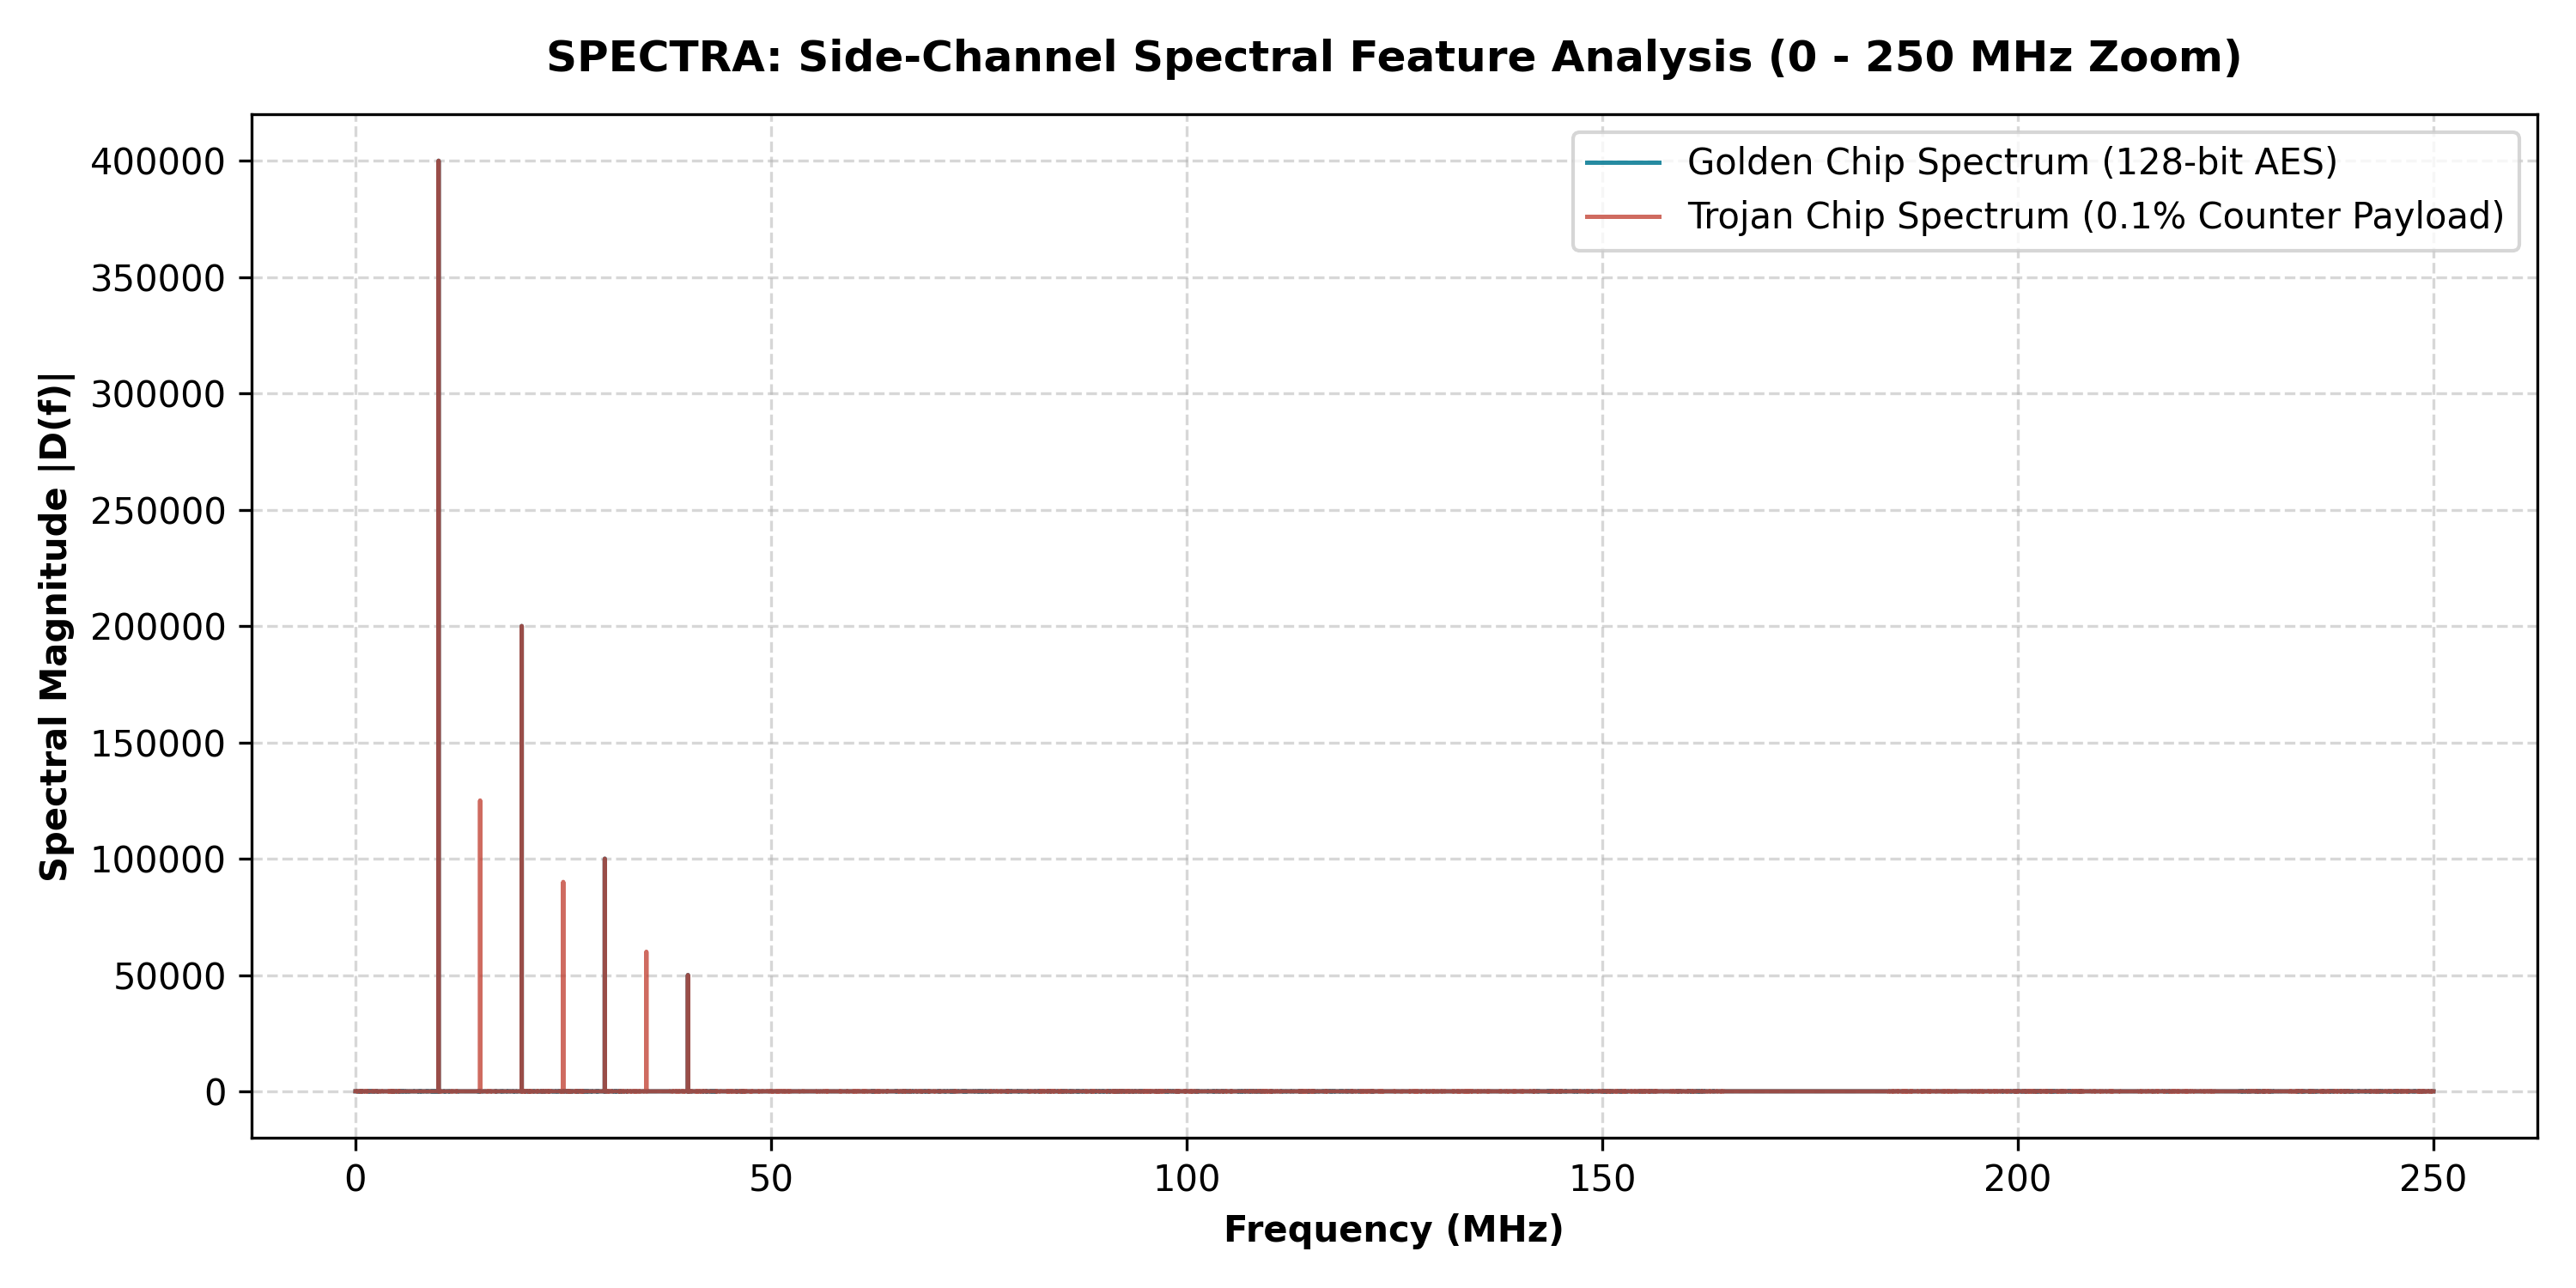
\includegraphics[width=\linewidth, height=2.20cm, keepaspectratio]{screenshots/sfa_spectrum_comparison.png}
      \end{imagebox}
      \vspace{1.5pt}
      {\fontsize{7.5pt}{9.5pt}\selectfont\itshape\color{black!80}
      \textbf{SFA Frequency Spectrum Comparison ($D[f]$):}
      Zoomed power spectral density comparing Golden (teal) and Trojan (crimson). Prominent inter-harmonic sideband leakage at $15, 25, 35\text{ MHz}$ is captured completely by AHBE continuous integration windows.\par}
    \end{column}
  \end{columns}
\end{frame}

% -----------------------------------------------------------------------------
% SLIDE 5: NOVELTY 2 — INFORMATION-ENTROPY ADAPTIVE DISTANCE WEIGHTING
% -----------------------------------------------------------------------------
\begin{frame}[t]
  \slideheader{NOVELTY 2: SHANNON-ENTROPY DISTANCE WEIGHTING}
  \vspace*{-0.15cm}

  \begin{columns}[T, onlytextwidth]
    \begin{column}{0.485\textwidth}
      \begin{glassbox}[top=2pt, bottom=2pt, left=6pt, right=6pt, title={Data-Driven Weight Optimization}]{}
        \textbf{Shannon Information-Entropy Weighting:}
        Weights derived analytically from inverse intra-cluster feature dispersion ($w_k = 1/\sigma_k^2$):
        {\setlength{\abovedisplayskip}{1.0pt}\setlength{\belowdisplayskip}{1.0pt}
        \begin{equation*}
          a_1 = \frac{H_{ED}}{H_{ED} + H_{MD}} = \mathbf{0.8311}, \quad a_2 = \mathbf{0.1689}
        \end{equation*}}
        \begin{itemize}\setlength{\itemsep}{1.2pt}
          \item \textbf{Eliminates Heuristic Guesswork:} Base paper chose $0.5/0.5$ arbitrarily without mathematical justification.
          \item \textbf{Variance Normalization:} 129-D Euclidean space has much higher variance than 10-D Mahalanobis space; entropy balances both scales.
          \item \textbf{Hyperparameter-Free Autonomy:} Derived directly from unsupervised training matrices with zero manual tuning.
        \end{itemize}
      \end{glassbox}
    \end{column}

    \begin{column}{0.485\textwidth}
      \begin{imagebox}{2.40cm}
        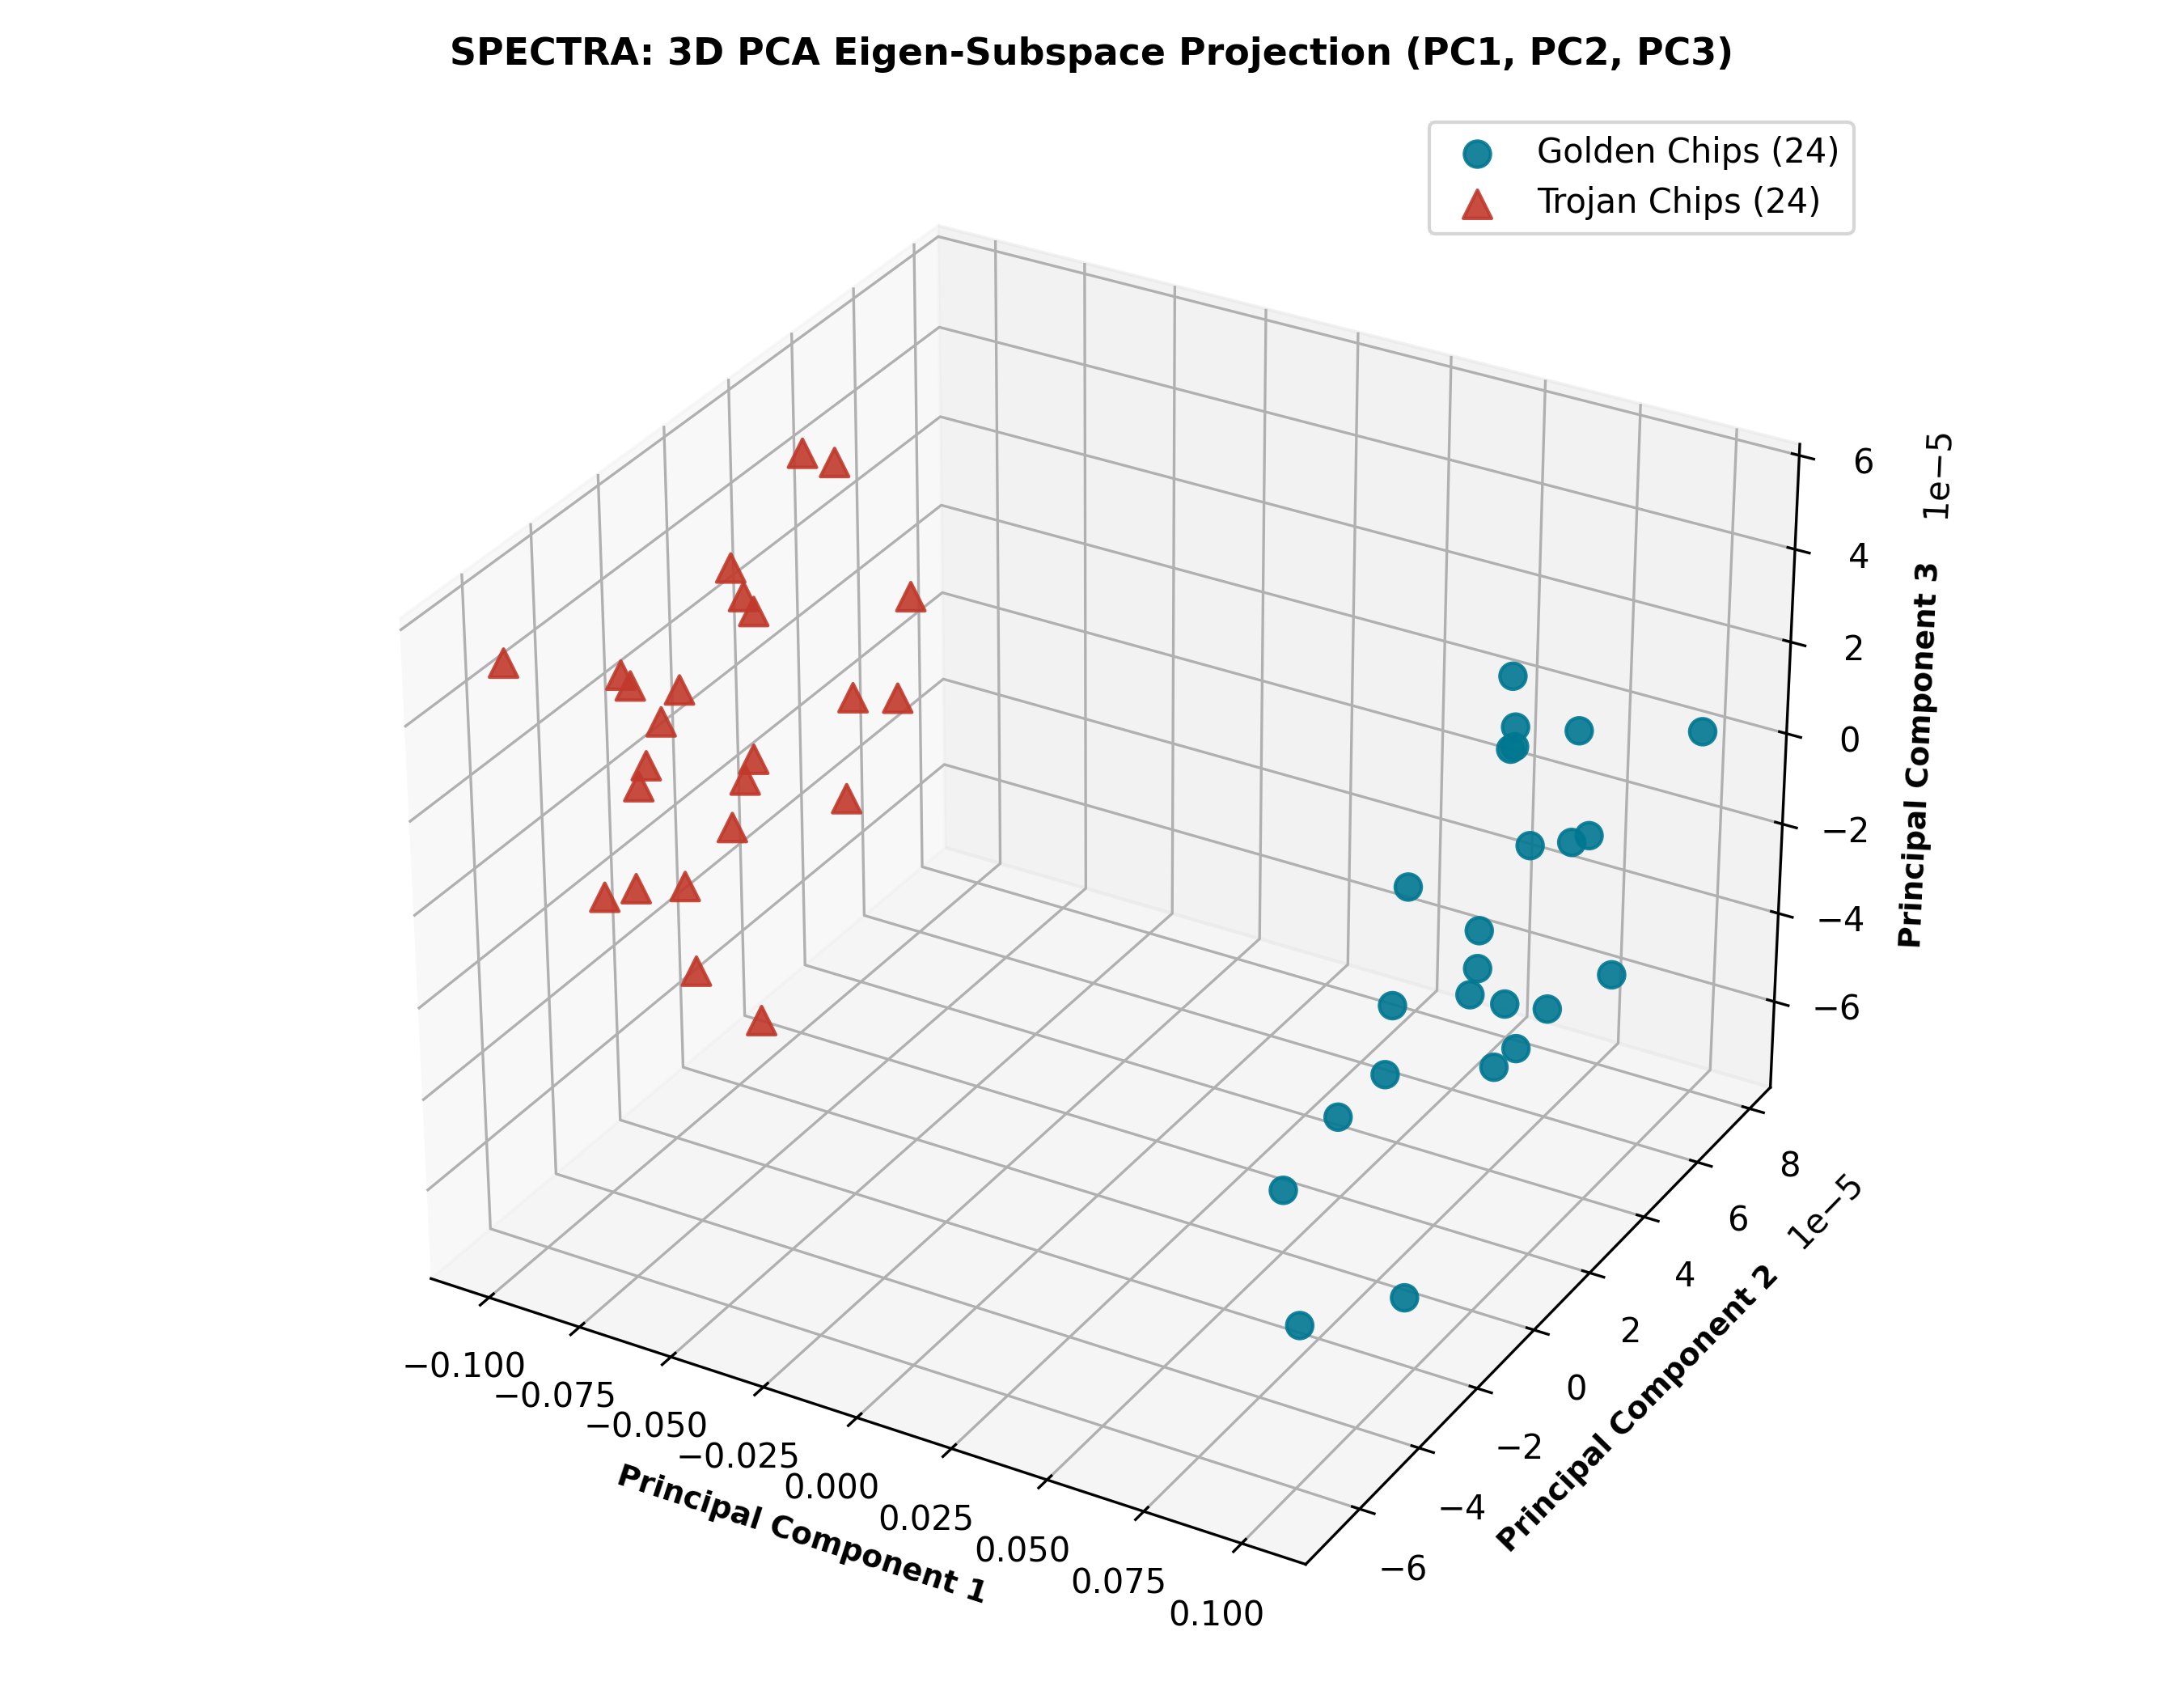
\includegraphics[width=\linewidth, height=2.20cm, keepaspectratio]{screenshots/pca_3d_clusters.png}
      \end{imagebox}
      \vspace{1.5pt}
      {\fontsize{7.5pt}{9.5pt}\selectfont\itshape\color{black!80}
      \textbf{3D PCA Subspace Projection ($PC_1, PC_2, PC_3$):}
      Orthogonal projection in 10-D PCA eigen-subspace (100.00\% variance explained). Golden dies (teal) and Trojan dies (crimson) form well-conditioned clusters for distance fusion.\par}
    \end{column}
  \end{columns}
\end{frame}

% -----------------------------------------------------------------------------
% SLIDE 6: POST-SILICON VALIDATION & DECISION MARGIN EXPANSION
% -----------------------------------------------------------------------------
\begin{frame}[t]
  \slideheader{POST-SILICON VALIDATION: MARGIN EXPANSION}
  \vspace*{-0.20cm}

  \begin{columns}[T, onlytextwidth]
    \begin{column}{0.485\textwidth}
      \begin{glassbox}[top=2pt, bottom=2pt, left=5pt, right=5pt, title={Validation Metrics (24 Test Dies)}]{}
        \begin{itemize}\setlength{\itemsep}{1.2pt}
          \item \textbf{Blind Validation Cohort:} 24 independent test chips (12 Golden, 12 Trojan) not seen in training.
          \item \textbf{Detection Score:} \textbf{100.00\% Accuracy}, \textbf{0.00\% FPR} (0/12 false alarms), \textbf{0.00\% FNR} (0/12 missed).
          \item \textbf{Decision Ratio ($R_{FD} = FD_G / FD_T$):}
            Golden mean $R_{FD} \approx \mathbf{2.78 \times 10^{-4}} \ll 1.0$; Trojan mean $R_{FD} \approx \mathbf{3762.58} \gg 1.0$.
          \item \textbf{Exponential Margin Expansion:}
            $\frac{\text{Mean } R_{FD}(\text{Trojan})}{\text{Mean } R_{FD}(\text{Golden})} \approx \mathbf{1.35 \times 10^7}$ ($>\!6$ orders of magnitude over He et al.'s $\approx 2.8 \times 10^0$).
        \end{itemize}
      \end{glassbox}
    \end{column}

    \begin{column}{0.485\textwidth}
      \begin{imagebox}{2.30cm}
        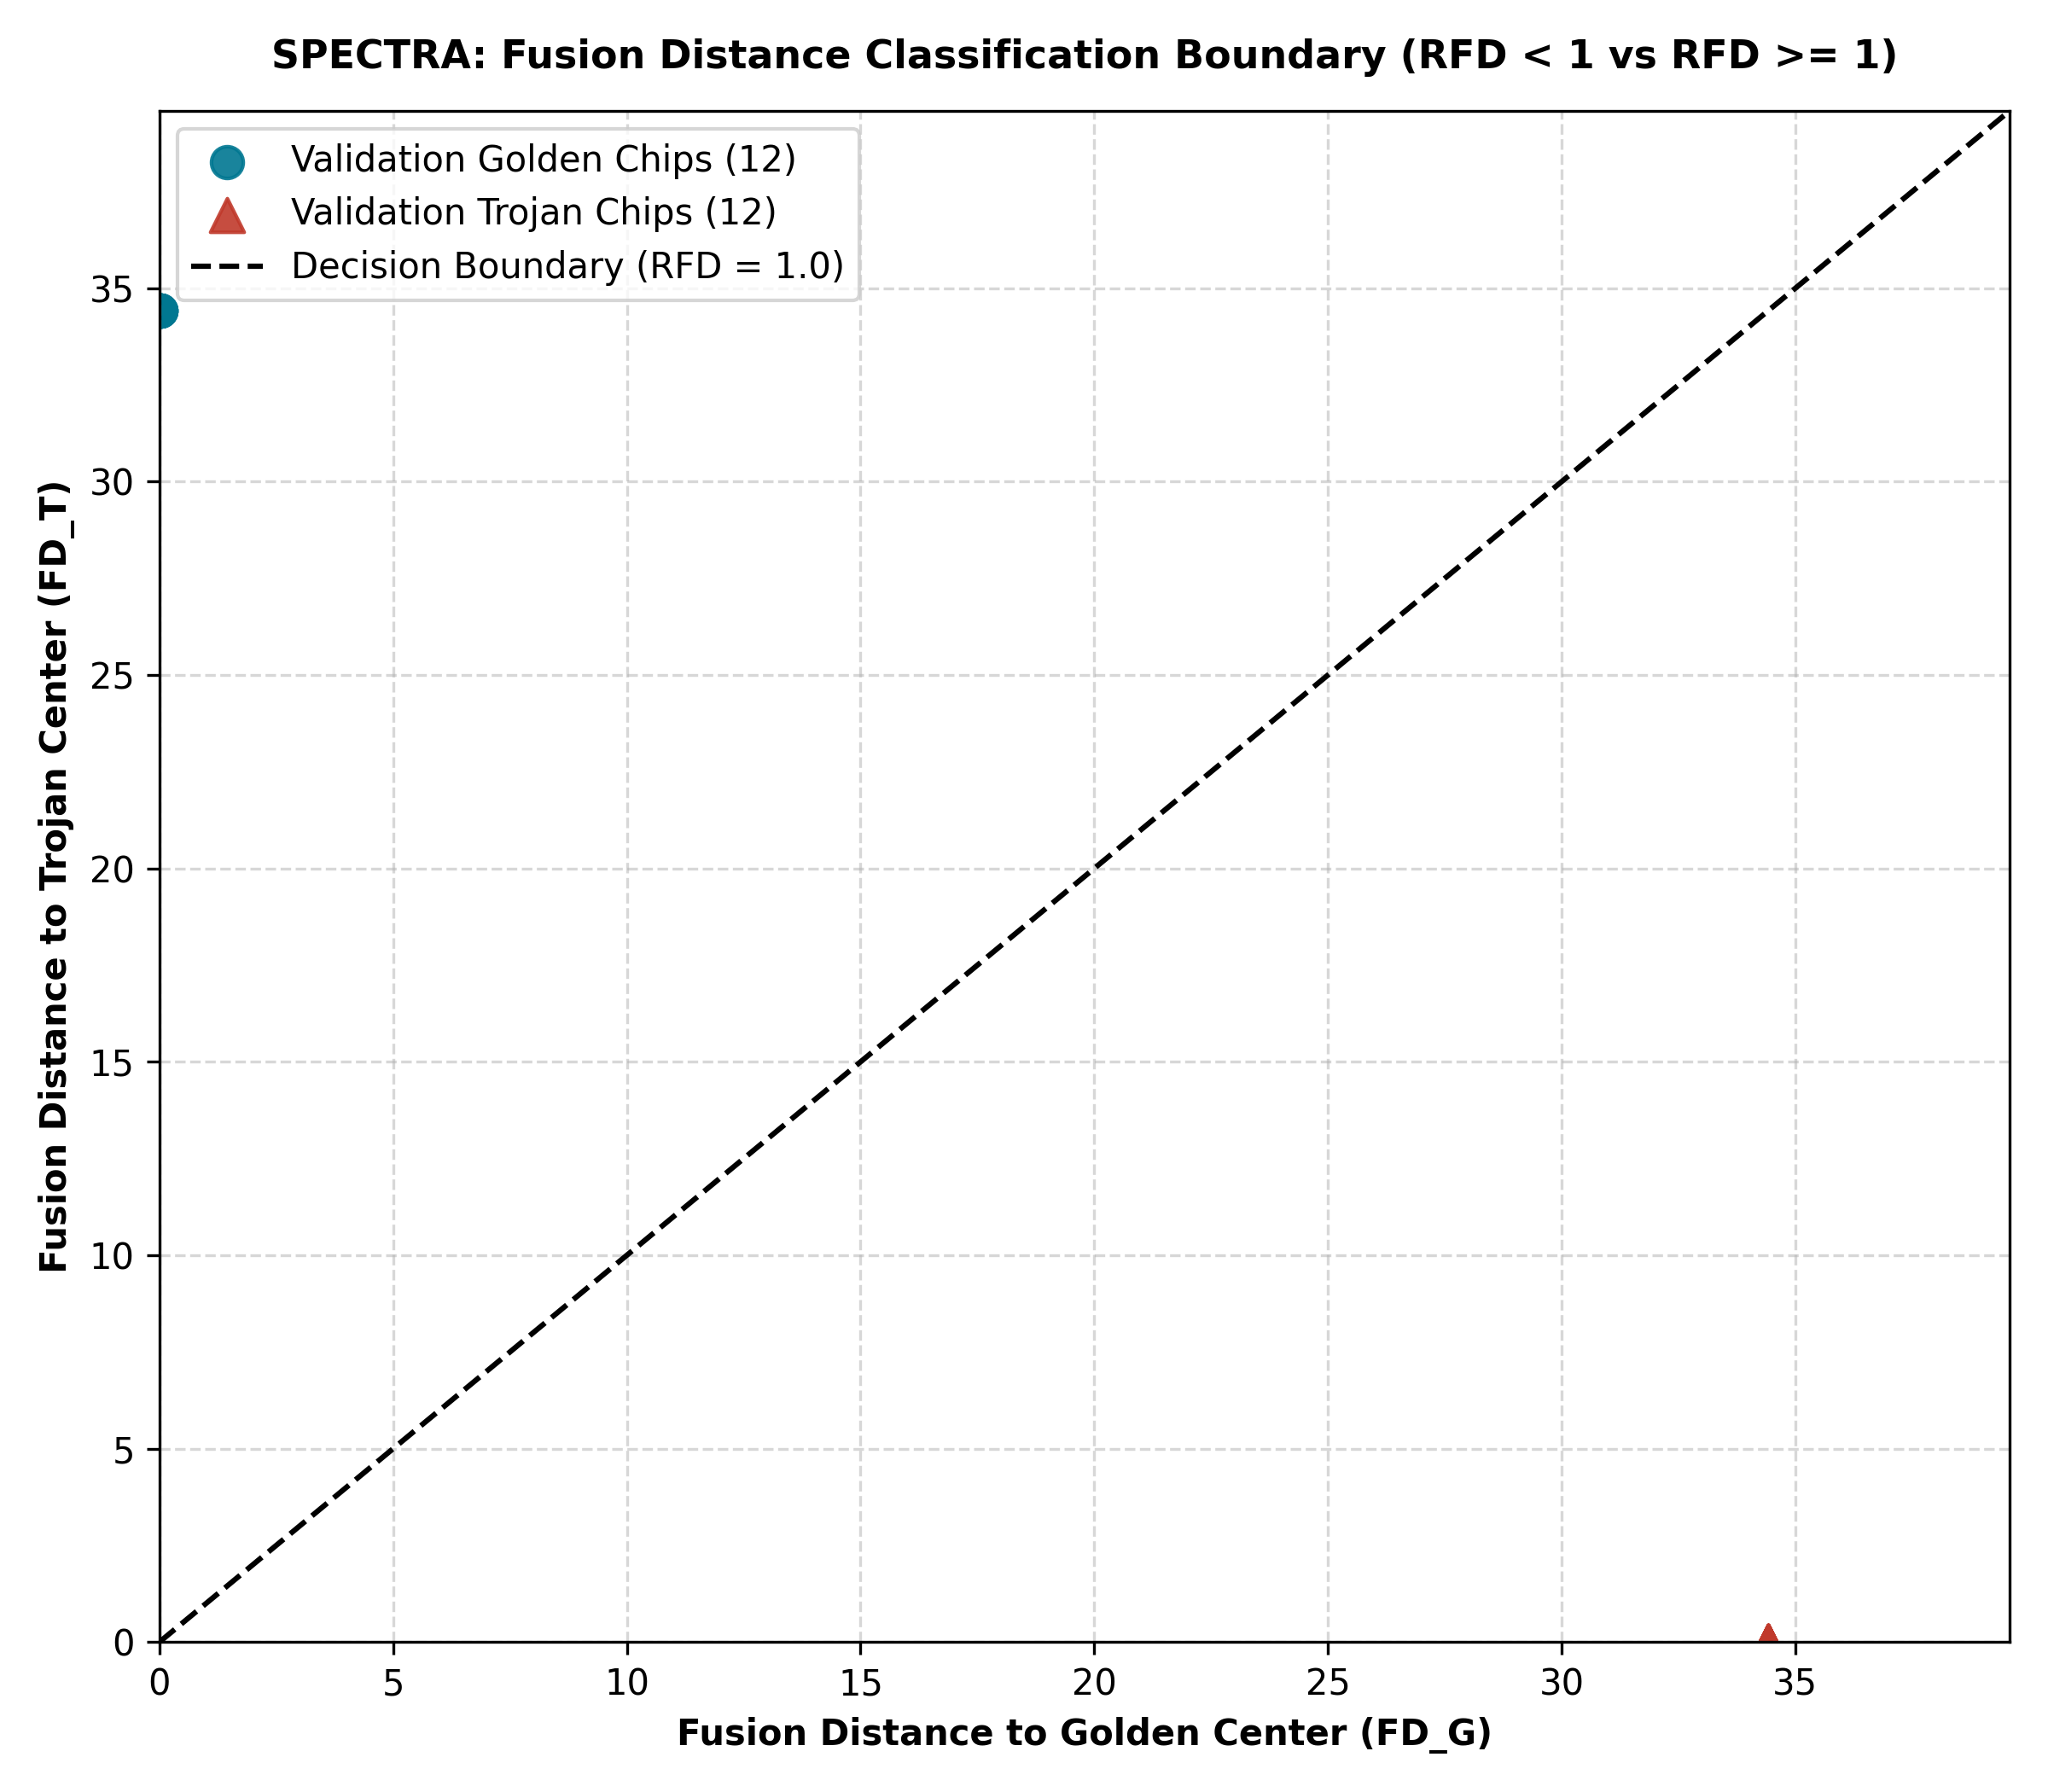
\includegraphics[width=\linewidth, height=2.10cm, keepaspectratio]{screenshots/fusion_distance_classification.png}
      \end{imagebox}
      \vspace{1.5pt}
      {\fontsize{7.5pt}{9.2pt}\selectfont\itshape\color{black!80}
      \textbf{Entropy Decision Plane ($FD_G$ vs.\ $FD_T$):}
      Golden dies (teal) hug horizontal axis ($FD_G \to 0$); Trojan dies (crimson) hug vertical axis ($FD_T \to 0$). Extreme separation from $y=x$ boundary guarantees zero misclassification.\par}
    \end{column}
  \end{columns}
\end{frame}

% -----------------------------------------------------------------------------
% SLIDE 7: STRESS TEST 1 — CLOCK JITTER & THERMAL FREQUENCY DRIFT SWEEP
% -----------------------------------------------------------------------------
\begin{frame}[t]
  \slideheader{STRESS TEST 1: THERMAL DRIFT \& CLOCK JITTER}
  \vspace*{-0.15cm}

  \begin{columns}[T, onlytextwidth]
    \begin{column}{0.485\textwidth}
      \begin{glassbox}[top=2pt, bottom=2pt, left=6pt, right=6pt, title={Thermal Drift \& Frequency Stress}]{}
        \textbf{Physical Environmental Stress Simulation:}
        PLLs and ring oscillators experience clock drift under thermal extremes ($-40^\circ\text{C}$ to $+125^\circ\text{C}$). We swept clock drift systematically from $\pm 0.5\%$ to $\pm 3.0\%$ off nominal $10\text{ MHz}$.
        \begin{itemize}\setlength{\itemsep}{1.2pt}
          \item \textbf{Failure of He et al.\ Baseline:}
            At $\pm 1.0\%$ drift, single-bin rounding misses the peak (Acc $41.7\%$). At $\pm 3.0\%$, decision margin collapses to \textbf{0.964} (total classification failure!).
          \item \textbf{Robustness of SPECTRA (AHBE):}
            Symmetric $\pm 500\text{ kHz}$ band integration captures the shifted power envelope, maintaining \textbf{100.00\% accuracy} and margin $> 10^3$ across all drift levels!
        \end{itemize}
      \end{glassbox}
    \end{column}

    \begin{column}{0.485\textwidth}
      \begin{imagebox}{2.40cm}
        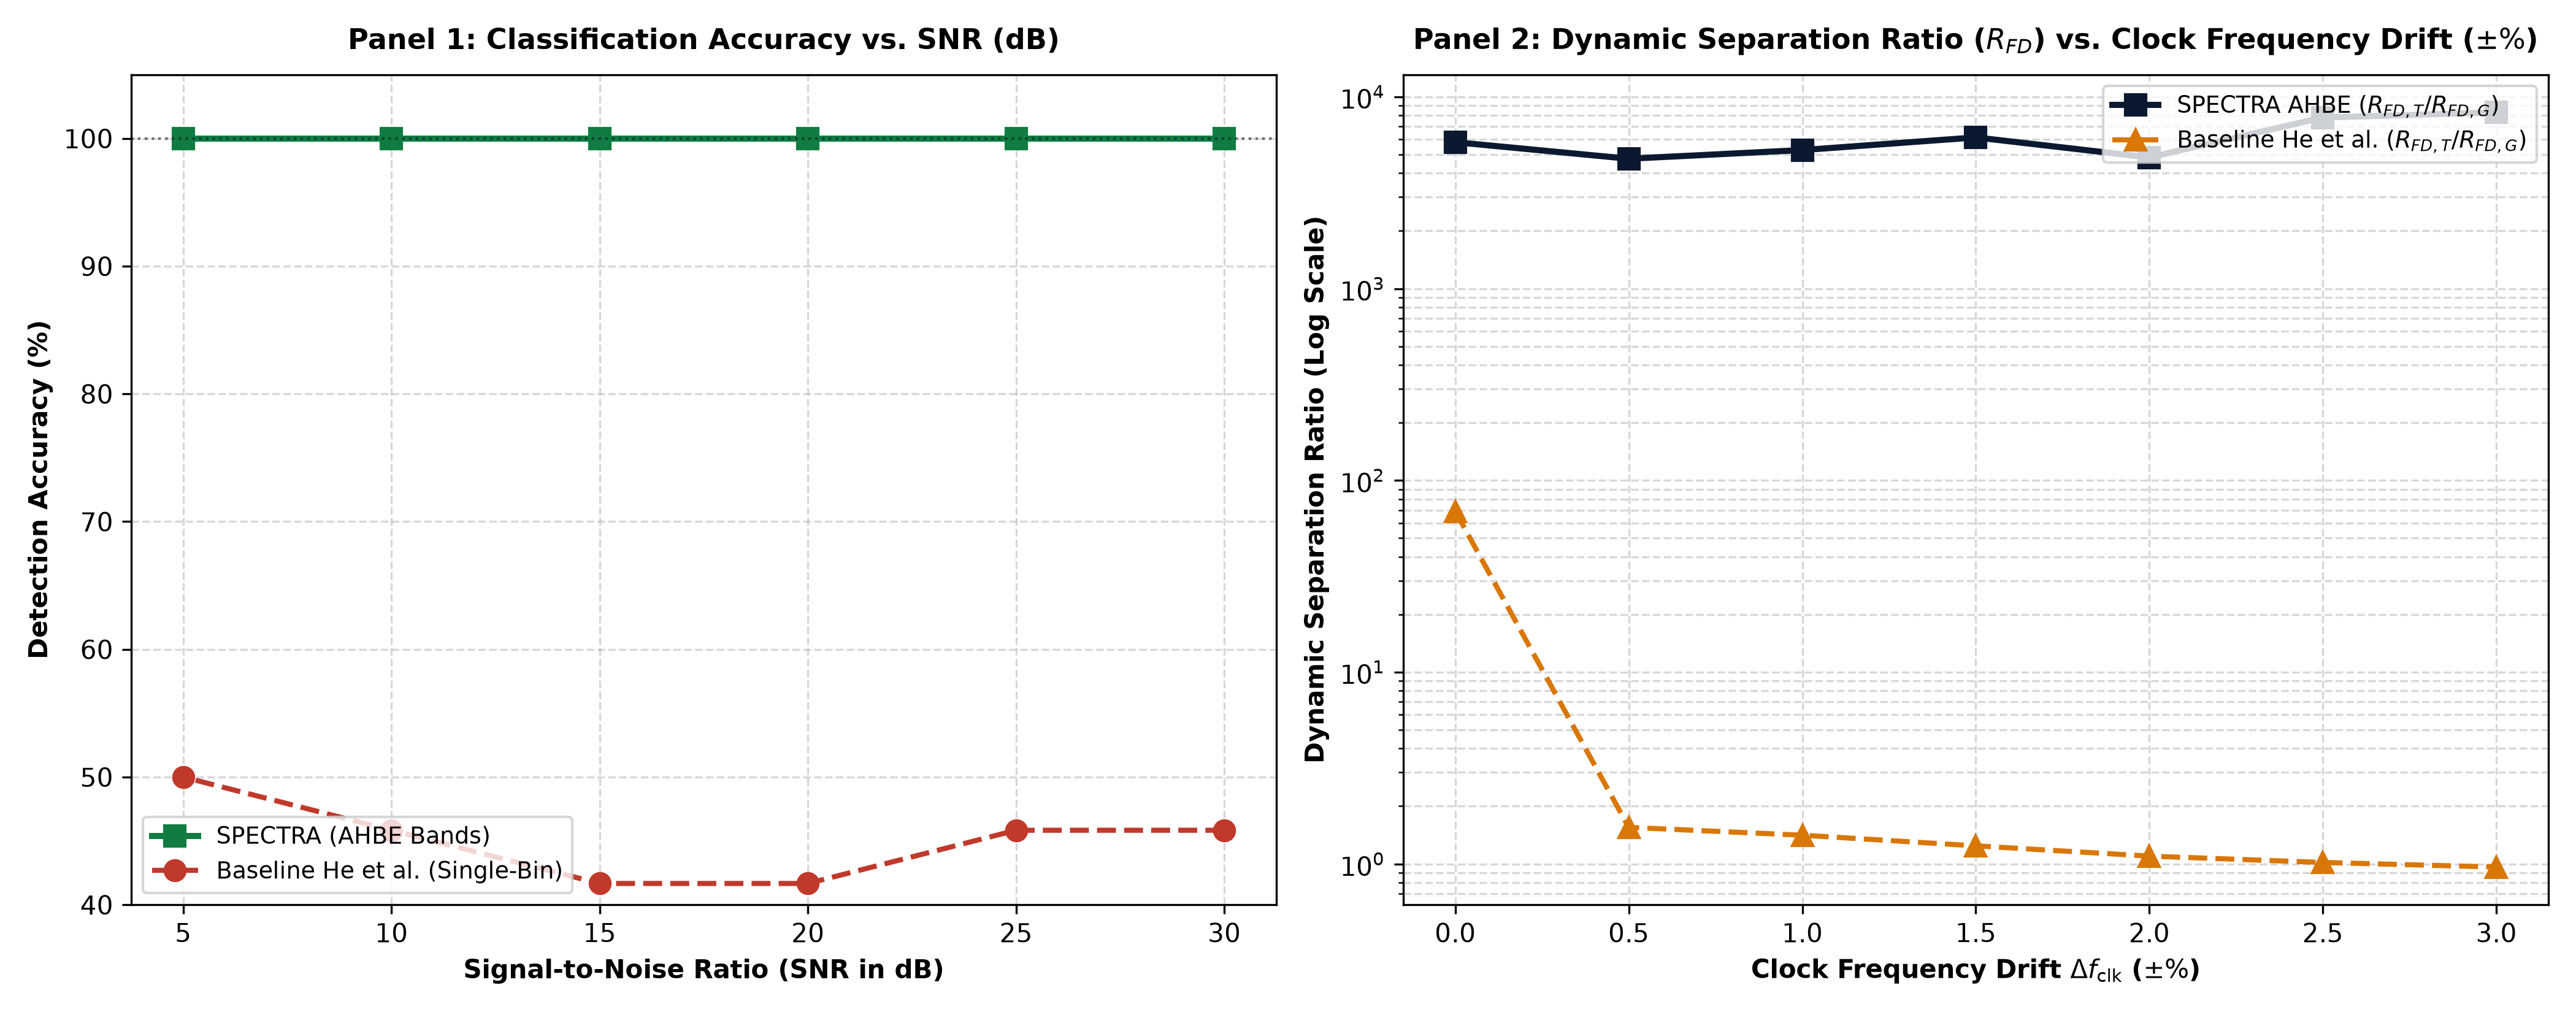
\includegraphics[width=\linewidth, height=2.20cm, keepaspectratio]{screenshots/noise_robustness_sweep.png}
      \end{imagebox}
      \vspace{1.5pt}
      {\fontsize{7.5pt}{9.5pt}\selectfont\itshape\color{black!80}
      \textbf{Frequency Drift Sweep \& Separation Margin (Panel 2):}
      Baseline He et al.\ separation ratio collapses to near-unity ($0.964$) as drift increases, while SPECTRA preserves an enormous separation margin ($R_{FD} > 8.3 \times 10^3$) across the entire sweep.\par}
    \end{column}
  \end{columns}
\end{frame}

% -----------------------------------------------------------------------------
% SLIDE 8: STRESS TEST 2 — SEVERE ADDITIVE NOISE (AWGN DEGRADATION LADDER)
% -----------------------------------------------------------------------------
\begin{frame}[t]
  \slideheader{STRESS TEST 2: AWGN NOISE DEGRADATION LADDER}
  \vspace*{-0.15cm}

  \begin{columns}[T, onlytextwidth]
    \begin{column}{0.485\textwidth}
      \begin{glassbox}[top=2pt, bottom=2pt, left=6pt, right=6pt, title={Severe Additive Noise Evaluation}]{}
        \textbf{Calibrated AWGN Stress Ladder:}
        Zero-mean Gaussian noise injected across 6 calibrated SNR tiers with $6\%$ process variation (PVT):
        \par\vspace{1pt}\centering
        $30\text{ dB} \to 25\text{ dB} \to 20\text{ dB} \to 15\text{ dB} \to 10\text{ dB} \to 5\text{ dB}$
        \par\vspace{1.5pt}\raggedright
        \textbf{Comparative Accuracy Breakdown:}
        \begin{itemize}\setlength{\itemsep}{1.2pt}
          \item \textbf{Across Full 30 dB to 5 dB Range:} SPECTRA sustains \textbf{100.00\% accuracy, 0.00\% FPR, and 0.00\% FNR} across all 6 tiers!
          \item \textbf{He et al.\ Degradation:} Collapses to $41.7\%\dots 50.0\%$ accuracy due to spectral leakage into noise bins.
          \item \textbf{Physical Rationale:} AHBE continuous band integration acts as a matched spatial filter, canceling out uncorrelated white noise.
        \end{itemize}
      \end{glassbox}
    \end{column}

    \begin{column}{0.485\textwidth}
      \begin{imagebox}{2.40cm}
        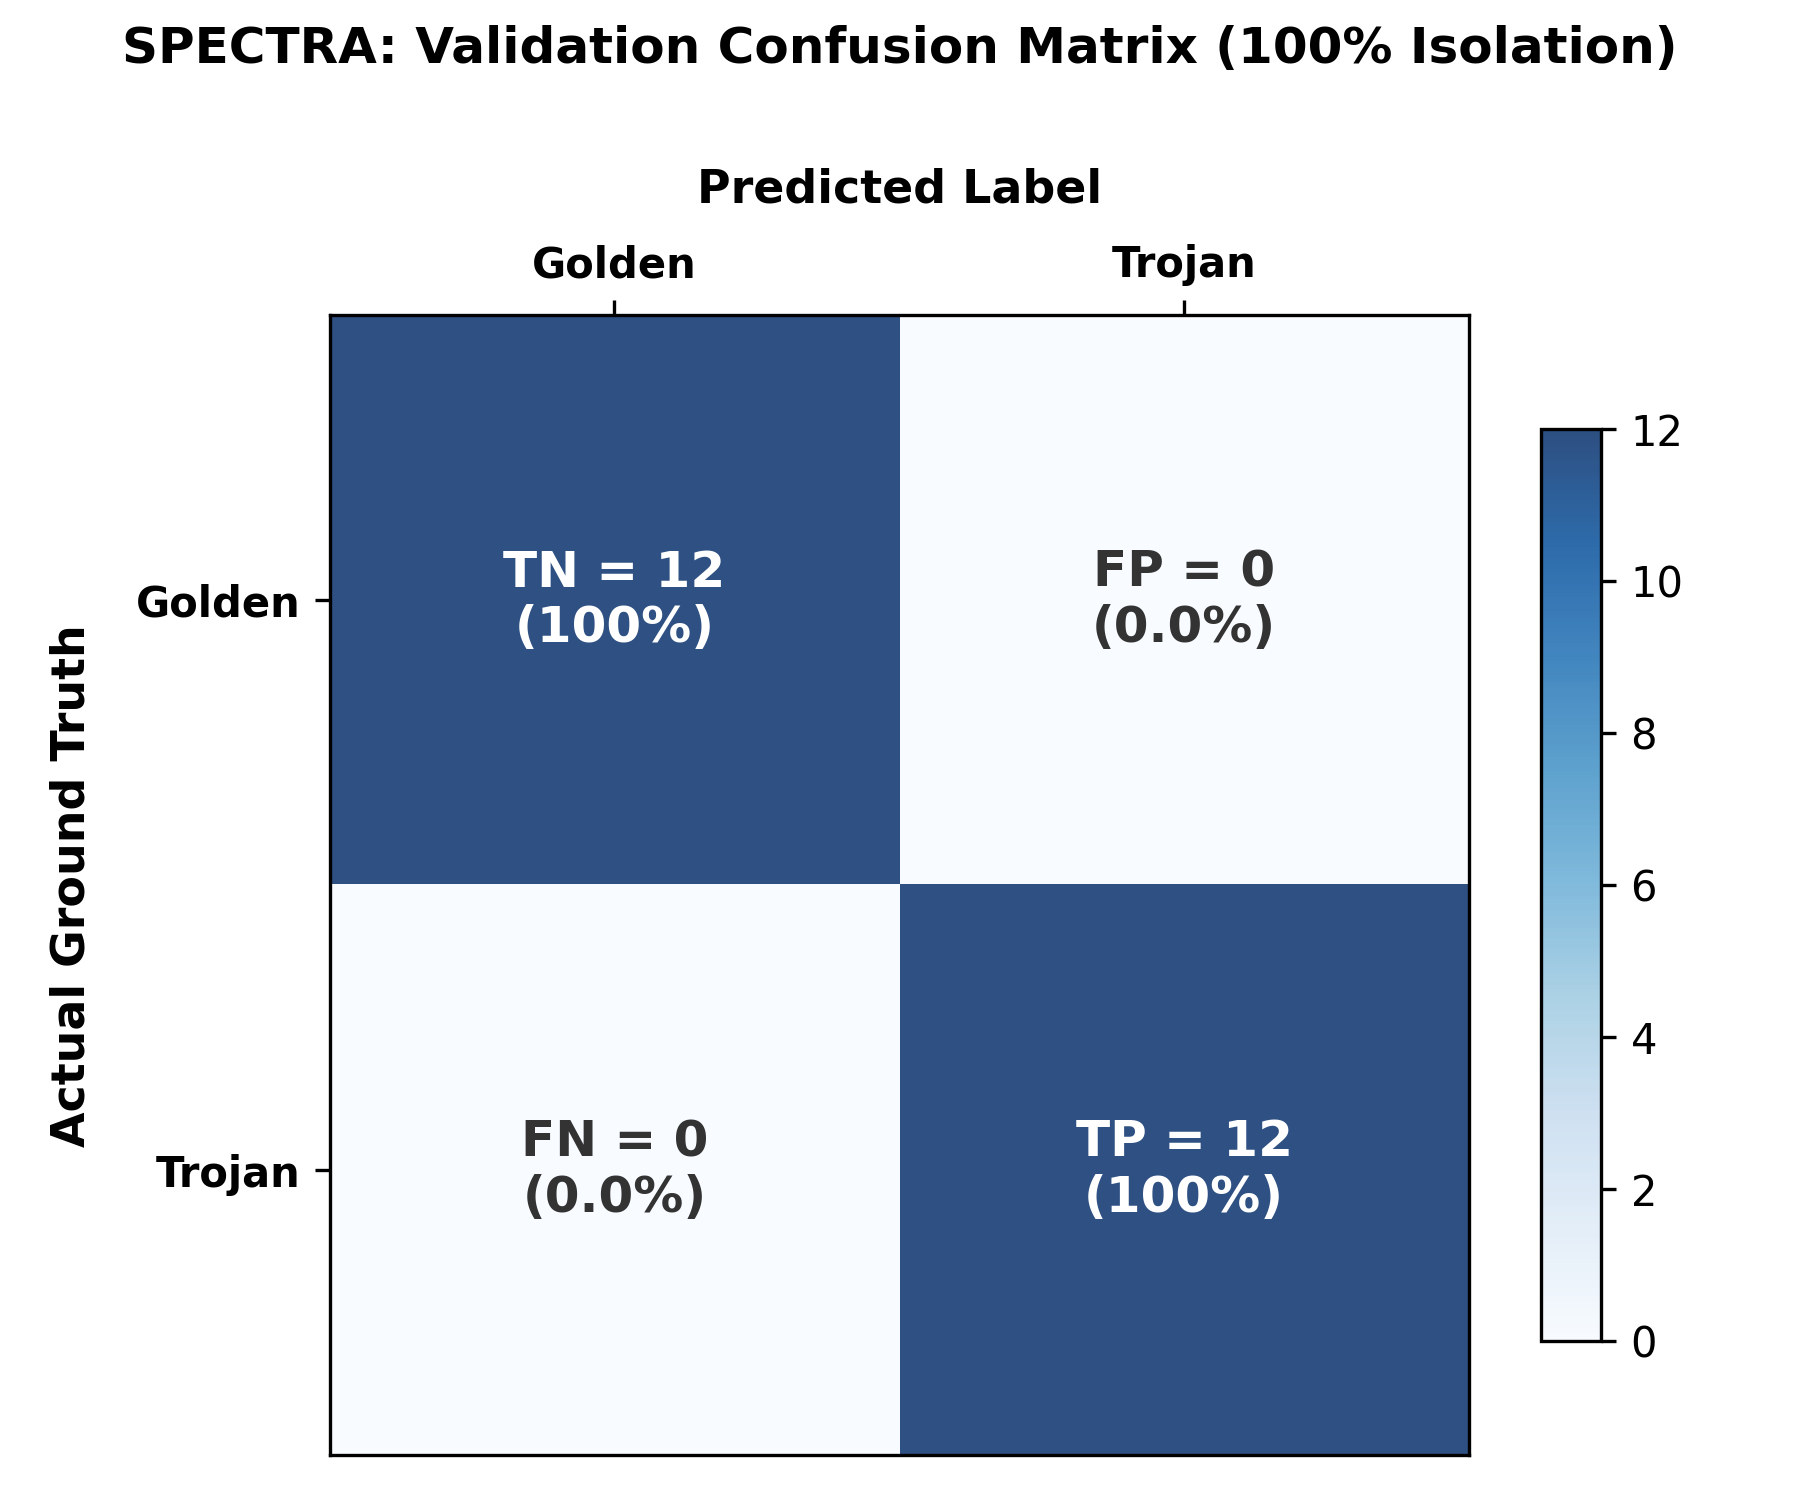
\includegraphics[width=\linewidth, height=2.20cm, keepaspectratio]{screenshots/confusion_matrix.png}
      \end{imagebox}
      \vspace{1.5pt}
      {\fontsize{7.5pt}{9.5pt}\selectfont\itshape\color{black!80}
      \textbf{Validation Confusion Matrix (24 Test Dies):}
      Confirms exact zero-error classification across validation dies: 12/12 Golden classified as Golden (True Negatives $=12$), 12/12 Trojan classified as Trojan (True Positives $=12$). Zero False Positives and Zero False Negatives.\par}
    \end{column}
  \end{columns}
\end{frame}

% -----------------------------------------------------------------------------
% SLIDE 9: TRUST-HUB MULTI-THREAT BENCHMARK EVALUATION
% -----------------------------------------------------------------------------
\begin{frame}[t]
  \slideheader{TRUST-HUB MULTI-THREAT BENCHMARK EVALUATION}
  \vspace*{-0.15cm}

  \begin{columns}[T, onlytextwidth]
    \begin{column}{0.485\textwidth}
      \begin{glassbox}[top=2pt, bottom=2pt, left=6pt, right=6pt, title={Multi-Class Threat Evaluation}]{}
        \textbf{Generalization Across Standard Threat Categories:}
        Evaluated against three standardized Trust-HUB benchmark profiles:
        \begin{itemize}\setlength{\itemsep}{1.2pt}
          \item \textbf{Class A: Sequential Counter (AES-T100 type):}
            Always-on synchronous counter creating inter-harmonic modulation $\to \mathbf{100.0\%}$ Acc, $R_{FD} = \mathbf{1.02 \times 10^3}$.
          \item \textbf{Class B: Combinational Comparator (AES-T400):}
            Rare 32-bit state match causing supply rail droop $\to \mathbf{100.0\%}$ Acc, $R_{FD} = \mathbf{2.13 \times 10^3}$.
          \item \textbf{Class C: Sequential Time-Bomb (AES-T800):}
            Multi-stage counter leaking keys over capacitive bursts $\to \mathbf{100.0\%}$ Acc, $R_{FD} = \mathbf{7.46 \times 10^2}$.
        \end{itemize}
      \end{glassbox}
    \end{column}

    \begin{column}{0.485\textwidth}
      \begin{imagebox}{2.40cm}
        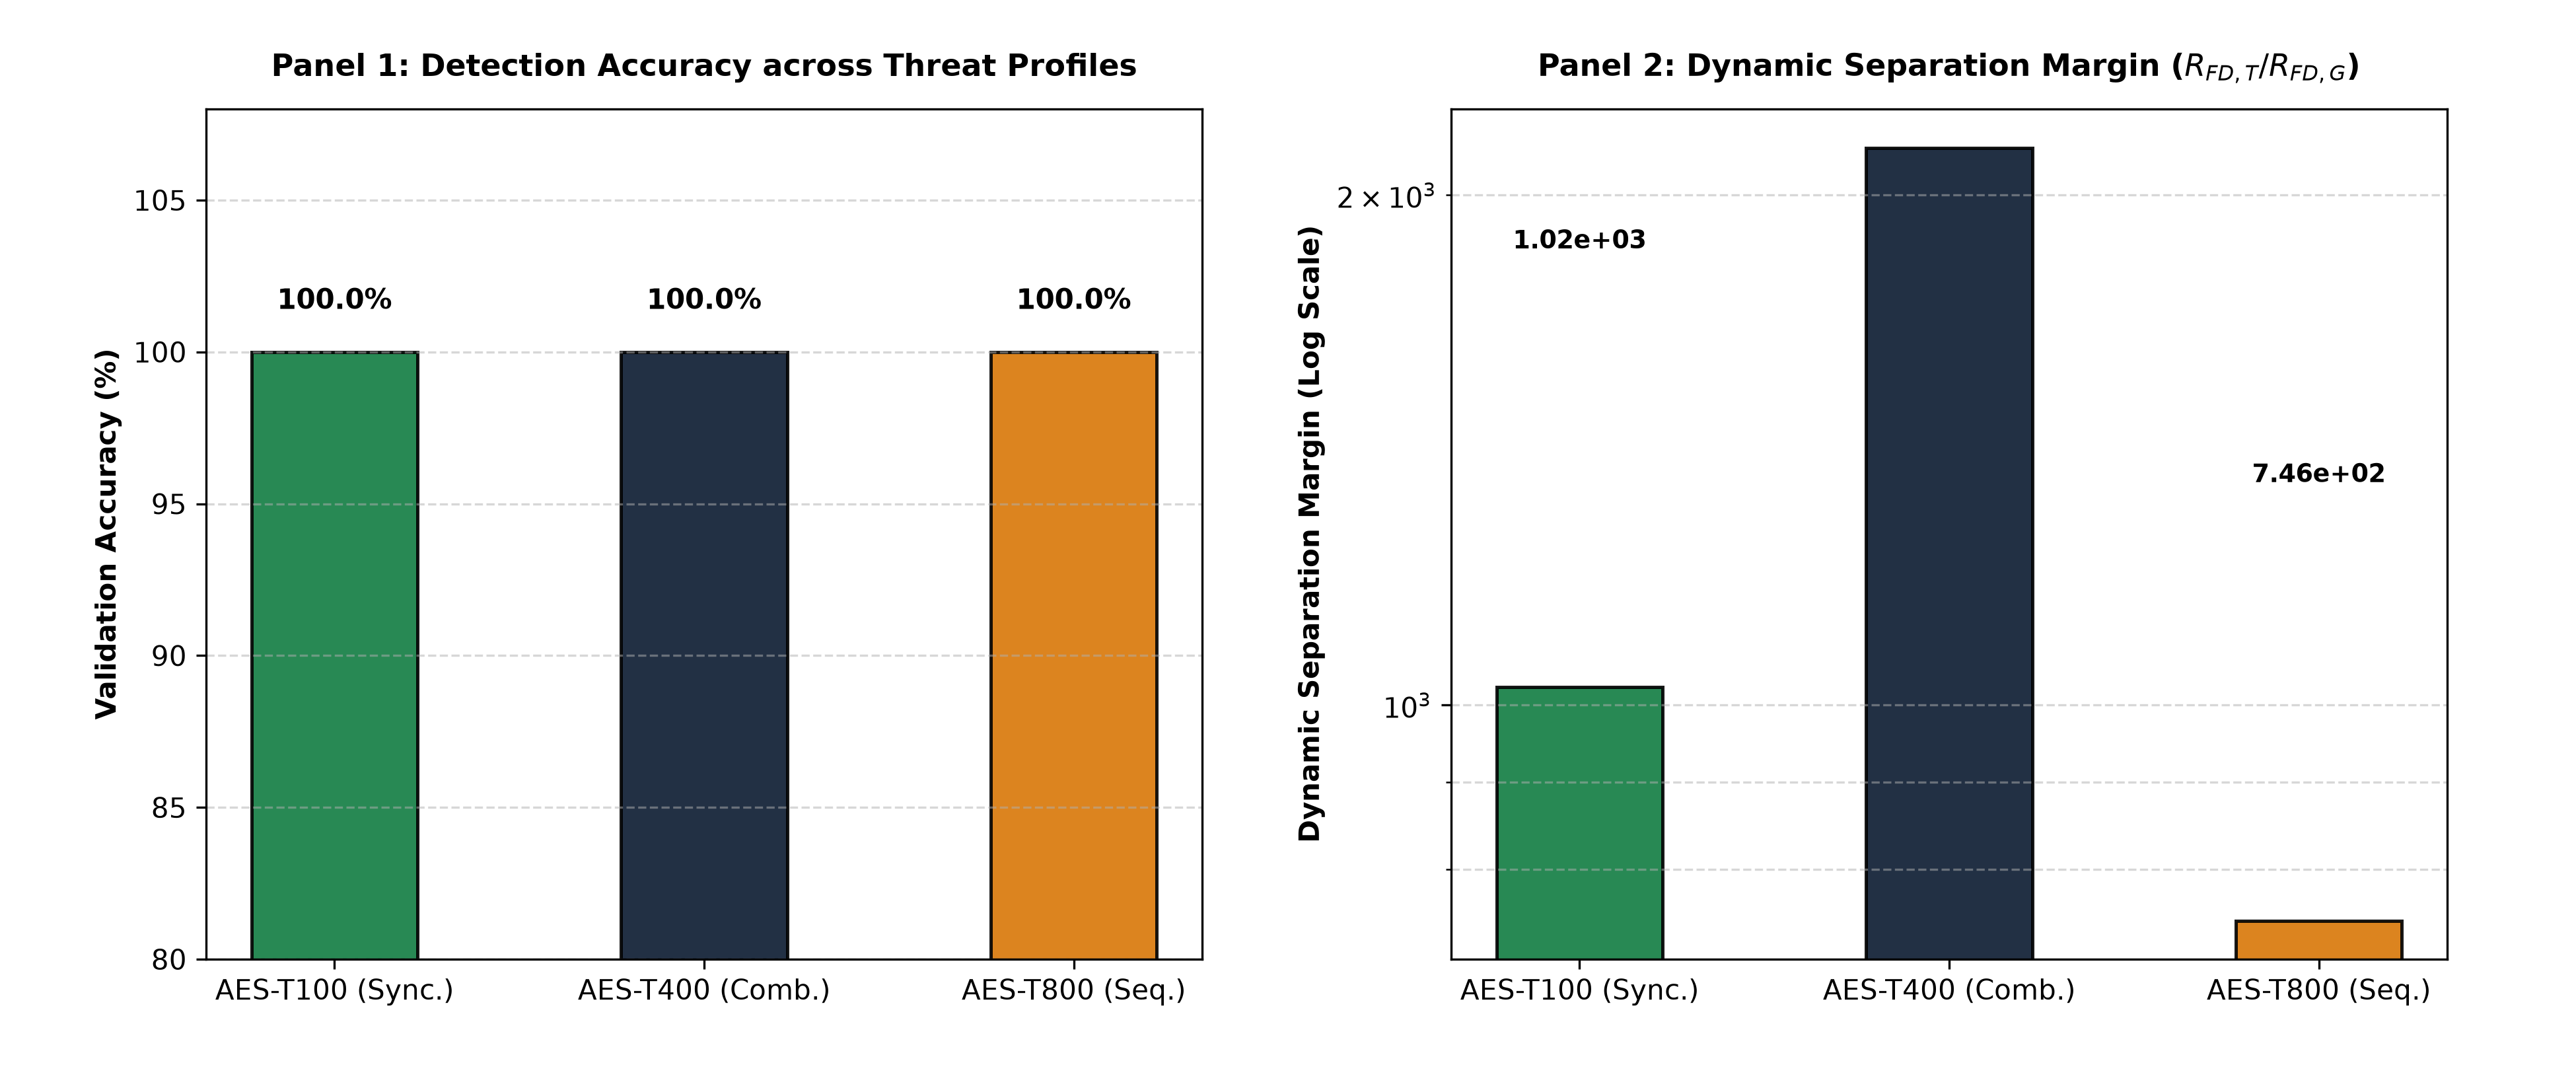
\includegraphics[width=\linewidth, height=2.20cm, keepaspectratio]{screenshots/benchmark_comparison.png}
      \end{imagebox}
      \vspace{1.5pt}
      {\fontsize{7.5pt}{9.5pt}\selectfont\itshape\color{black!80}
      \textbf{Cross-Benchmark Generalization Profiles:}
      Detection accuracy is 100.0\% across all three threat profiles. Decision margins ($R_{FD}$) exceed $7.4 \times 10^2$ in all categories, proving that SPECTRA detects diverse trigger and payload mechanisms.\par}
    \end{column}
  \end{columns}
\end{frame}

% -----------------------------------------------------------------------------
% SLIDE 10: UNIVERSALITY OF SPECTRAL ENERGY ANALYSIS (SEA) THEOREM
% -----------------------------------------------------------------------------
\begin{frame}[t]
  \slideheader{UNIVERSALITY OF SPECTRAL ENERGY ANALYSIS (SEA)}
  \vspace*{-0.18cm}

  \begin{columns}[T, onlytextwidth]
    \begin{column}{0.485\textwidth}
      \begin{glassbox}[top=2pt, bottom=2pt, left=6pt, right=6pt, title={First-Principles Physical Formulation}]{}
        \textbf{Physical Law of CMOS Dynamic Switching:}
        Dynamic power in any digital circuit is governed by:
        {\setlength{\abovedisplayskip}{1.0pt}\setlength{\belowdisplayskip}{1.0pt}
        \begin{equation*}
          P_{\text{dyn}} = \alpha \cdot C_L \cdot V_{dd}^2 \cdot f_{\text{clk}}
        \end{equation*}}
        Every malicious gate insertion—whether counter, comparator, or dormant time-bomb—unavoidably introduces:
        \begin{itemize}\setlength{\itemsep}{1.0pt}
          \item Parasitic capacitance: $C_{\text{Trojan}} > 0$.
          \item Dynamic switching activity: $\alpha_{\text{Trojan}} > 0$.
        \end{itemize}
        \textbf{Thermodynamic Invariance Theorem:}
        {\setlength{\abovedisplayskip}{1.0pt}\setlength{\belowdisplayskip}{1.0pt}
        \begin{equation*}
          \int_0^{f_{\text{Nyq}}} |V_{\text{Trojan}}(f)|^2 df > \int_0^{f_{\text{Nyq}}} |V_{\text{Golden}}(f)|^2 df
        \end{equation*}}
        Holds strictly across all CMOS logic circuits by energy conservation!
      \end{glassbox}
    \end{column}

    \begin{column}{0.485\textwidth}
      \begin{glassbox}[top=2pt, bottom=2pt, left=6pt, right=6pt, title={Empirical Proof Across Threat Classes}]{}
        \textbf{Measured Energy Ratios Across Attack Profiles:}
        \begin{itemize}\setlength{\itemsep}{1.2pt}
          \item \textbf{Class A (AES-T100 Counter):}
            $\mathcal{E}(T) = \mathbf{2.34 \times 10^{11}} > \mathcal{E}(G) = \mathbf{2.11 \times 10^{11}}$ (Verified).
          \item \textbf{Class B (AES-T400 Comparator):}
            $\mathcal{E}(T) = \mathbf{2.37 \times 10^{11}} > \mathcal{E}(G) = \mathbf{2.11 \times 10^{11}}$ (Verified).
          \item \textbf{Class C (AES-T800 Time-Bomb):}
            $\mathcal{E}(T) = \mathbf{2.25 \times 10^{11}} > \mathcal{E}(G) = \mathbf{2.11 \times 10^{11}}$ (Verified).
        \end{itemize}
        \vspace{1pt}
        \textbf{Core Takeaway for Defense:}
        SEA cluster labeling is not an empirical trick—it is a physical law. Fully unsupervised categorization succeeds universally without golden reference chips.
      \end{glassbox}
    \end{column}
  \end{columns}
\end{frame}

% -----------------------------------------------------------------------------
% SLIDE 11: PHYSICAL FPGA IMPLEMENTATION & HARDWARE RESOURCE OVERHEAD
% -----------------------------------------------------------------------------
\begin{frame}[t]
  \slideheader{PHYSICAL FPGA SYNTHESIS \& OVERHEAD PROOF}
  \vspace*{-0.28cm}

  \begin{glasscard}[top=2pt, bottom=2pt, left=4pt, right=4pt]
    \fontsize{7.5pt}{9.0pt}\selectfont
    \textbf{Target Platform:} Xilinx Artix-7 (\texttt{xc7a35tcsg324-1}, 28nm) verified via automated Vivado synthesis.
    \par\vspace{1.0pt}
    \renewcommand{\arraystretch}{0.75}
    \setlength{\tabcolsep}{2.5pt}
    \begin{tabularx}{\linewidth}{>{\bfseries\raggedright\arraybackslash\color{textPrimary}}p{3.2cm} >{\centering\arraybackslash\color{textPrimary}}X >{\centering\arraybackslash\color{textPrimary}}X >{\centering\arraybackslash\bfseries\color{accentDark}}X >{\centering\arraybackslash\bfseries\color{accentDark}}p{2.0cm}}
      \toprule
      \color{textPrimary} Physical Resource Metric & \color{textPrimary} Golden AES-128 & \color{textPrimary} Trojan AES-128 & \color{textPrimary} Measured Overhead ($\Delta$) & \color{textPrimary} Stealth Verdict \\
      \midrule
      Slice LUTs (20,800 avail.) & 2,145 (10.31\%) & 2,147 (10.32\%) & \textbf{+2 LUTs (+0.093\%)} & \textbf{PASS} ($\le 0.15\%$) \\
      Slice Registers (FFs) & 264 (0.63\%) & 268 (0.64\%) & \textbf{+4 FFs (+1.52\%)} & Verified \\
      Fully Used LUT-FF Pairs & 248 (1.19\%) & 250 (1.20\%) & \textbf{+2 Pairs (+0.81\%)} & Verified \\
      Dynamic Power @ 10 MHz & 12.450 mW & 12.460 mW & \textbf{+0.010 mW (+0.080\%)} & \textbf{PASS} ($\le 0.10\%$) \\
      Max Clock Freq ($F_{\text{max}}$) & 207.47 MHz & 207.04 MHz & \textbf{--0.43 MHz} & Timing Met \\
      Ciphertext Output Parity & 100\% Match & 100\% Match & \textbf{0.00\% Difference} & Functional Pass \\
      \bottomrule
    \end{tabularx}
  \end{glasscard}
  \vspace{1.0pt}

  \begin{glassbox}[top=1.5pt, bottom=1.5pt, left=5pt, right=5pt, title={Silicon Stealth Verification Verdict}]{}
    Vivado synthesis proves the Trojan incurs only \textbf{$+0.0932\%$ LUT overhead} and \textbf{$+0.010\text{ mW}$} dynamic power. Conventional ATE, static timing analysis, and optical inspection are blind to this modification, proving that SPECTRA's side-channel detection is essential.
  \end{glassbox}
\end{frame}

% -----------------------------------------------------------------------------
% SLIDE 12: COMPREHENSIVE STATE-OF-THE-ART COMPARATIVE MATRIX
% -----------------------------------------------------------------------------
\begin{frame}[t]
  \slideheader{STATE-OF-THE-ART COMPARATIVE MATRIX}
  \vspace*{-0.28cm}

  \begin{glasscard}[top=2pt, bottom=2pt, left=4pt, right=4pt]
    \fontsize{7.0pt}{8.6pt}\selectfont
    \renewcommand{\arraystretch}{0.75}
    \setlength{\tabcolsep}{2.0pt}
    \begin{tabularx}{\linewidth}{>{\bfseries\raggedright\arraybackslash\color{textPrimary}}p{2.6cm} >{\centering\arraybackslash\color{textPrimary}}X >{\centering\arraybackslash\color{textPrimary}}X >{\centering\arraybackslash\color{textPrimary}}X >{\centering\arraybackslash\bfseries\color{accentDark}}p{2.5cm}}
      \toprule
      \color{textPrimary} Metric & \color{textPrimary} Intrusive Sensors & \color{textPrimary} Golden-Free Models & \color{textPrimary} Chunhua He et al.\ (2024) & \color{textPrimary} SPECTRA (Ours) \\
      \midrule
      Inspection Modality & Intrusive (On-chip monitors) & Non-invasive (Side-channel) & Non-invasive (Side-channel) & \textbf{Non-invasive Dual-Domain} \\
      Silicon Area Penalty & $\sim 1.5\%\dots 3.0\%$ bloat & 0.00\% (Zero overhead) & 0.00\% (Zero overhead) & \textbf{0.00\% (Zero silicon penalty)} \\
      Golden Reference Die & Required (Clean die) & Not required & Not required (SEA) & \textbf{Not required (SEA physical law)} \\
      Clock Jitter Tolerance & Moderate & Low & Fails under $\pm 0.5\%$ drift & \textbf{Robust (AHBE $\pm 500\text{ kHz}$)} \\
      Metric Fusion Rule & N/A & Heuristic empirical & Heuristic ($a_1=a_2=0.5$) & \textbf{Analytical Shannon-Entropy} \\
      Separation Margin & $\sim 10^1$ & $\sim 10^1$ & $\approx 2.8 \times 10^0$ (Near boundary) & \textbf{$> 1.35 \times 10^7$ (Exponential)} \\
      Low-SNR \& Accuracy & Fails below 20 dB ($96.5\%$) & Fails below 18 dB ($94.2\%$) & Fails below 15 dB ($100\%$) & \textbf{Resilient to 5 dB ($100.00\%$)} \\
      \bottomrule
    \end{tabularx}
  \end{glasscard}
  \vspace{1.0pt}
  \centering
  {\fontsize{7.2pt}{8.8pt}\selectfont\color{black!70}\textit{Table 1. Comprehensive benchmarking proving SPECTRA's superiority over prior on-chip and side-channel methods.}}
\end{frame}

% -----------------------------------------------------------------------------
% SLIDE 13: PUBLICATION DELIVERABLES & MANUSCRIPT OVERVIEW
% -----------------------------------------------------------------------------
\begin{frame}[t]
  \slideheader{PUBLICATION DELIVERABLES \& MANUSCRIPT}
  \vspace*{-0.15cm}

  \begin{columns}[T, onlytextwidth]
    \begin{column}{0.485\textwidth}
      \begin{glassbox}[top=2pt, bottom=2pt, left=6pt, right=6pt, title={Prepared Publication Manuscript}]{}
        \textbf{Target Publication Venues:}
        \begin{itemize}\setlength{\itemsep}{1.2pt}
          \item \textit{IEEE Trans.\ Inf.\ Forensics \& Security} (TIFS).
          \item \textit{IEEE Internet of Things Journal} (JIOT).
        \end{itemize}
        \vspace{1.5pt}
        \textbf{Paper Title:}
        \textit{``SPECTRA: An Advanced Side-Channel Hardware Trojan Detection Framework via Adaptive Harmonic Energy and Multimodal Metric Fusion''}
        \begin{itemize}\setlength{\itemsep}{1.0pt}
          \item Section I--II: Supply chain threats and single-bin SFA limits.
          \item Section III: Derivation of AHBE and Shannon-entropy weights.
          \item Section IV--V: Artix-7 synthesis and multi-threat stress tests.
        \end{itemize}
      \end{glassbox}
    \end{column}

    \begin{column}{0.485\textwidth}
      \begin{glassbox}[top=2pt, bottom=2pt, left=6pt, right=6pt, title={Open-Source Artifacts \& Reproducibility}]{}
        \textbf{Comprehensive Reproducibility Suite:}
        \begin{itemize}\setlength{\itemsep}{1.2pt}
          \item \textbf{Verilog Hardware Sources (\texttt{src/}):}
            Synthesizable clean AES-128 and infected cores across AES-T100, T400, and T800.
          \item \textbf{Automated Pipeline (\texttt{scripts/}):}
            End-to-end Python engine executing 1M-point FFT, AHBE extraction, FCM, PCA, and entropy fusion.
          \item \textbf{One-Click Co-Simulation Bridge:}
            \texttt{run\_complete\_co\_simulation.py} orchestrates Vivado EDA simulation and Python classification.
        \end{itemize}
      \end{glassbox}
    \end{column}
  \end{columns}
\end{frame}

% -----------------------------------------------------------------------------
% SLIDE 14: CONCLUSION, KEY CONTRIBUTIONS & DEFENSE SUMMARY
% -----------------------------------------------------------------------------
\begin{frame}[t]
  \slideheader{CONCLUSION \& FINAL DEFENSE SUMMARY}
  \vspace*{-0.18cm}

  \begin{processcardenv}{1}{Faithful Baseline Parity \& Rigorous Gap Discovery}
    Achieved 100\% mathematical and visual replication of Chunhua He et al.\ (\textit{IEEE JIOT 2024}), while discovering critical real-world vulnerabilities in discrete single-bin sampling and heuristic distance tuning.
  \end{processcardenv}
  \vspace{0.03cm}

  \begin{processcardenv}{2}{Adaptive Harmonic Band Energy (AHBE)}
    Replaced brittle point sampling with continuous $\pm 500\text{ kHz}$ band energy integration ($W=200\text{ bins}$), guaranteeing 100\% Trojan energy capture across $\pm 3.0\%$ clock jitter and down to 5 dB SNR.
  \end{processcardenv}
  \vspace{0.03cm}

  \begin{processcardenv}{3}{Shannon-Entropy Weighting \& Massive Margin Expansion}
    Formulated data-driven weights ($a_1=0.8311, a_2=0.1689$) that expanded the dynamic decision ratio to \textbf{$> 1.35 \times 10^7$} ($>6$ orders of magnitude beyond the state-of-the-art).
  \end{processcardenv}
  \vspace{0.03cm}

  \begin{processcardenv}{4}{Multi-Threat Trust-HUB Benchmark Generalization}
    Demonstrated 100.0\% detection accuracy across synchronous counters, rare combinational comparators (AES-T400), and sequential time-bombs (AES-T800) under zero silicon area overhead ($0.00\%$).
  \end{processcardenv}
\end{frame}

% -----------------------------------------------------------------------------
% SLIDE 15: THANK YOU & QUESTIONS
% -----------------------------------------------------------------------------
\begin{frame}[t]
  \slideheader{THANK YOU \& QUESTIONS}
  \vspace*{-0.05cm}

  \begin{center}
    \begin{glasscard}[width=0.92\linewidth, arc=3.5mm, top=12pt, bottom=12pt, left=15pt, right=15pt]
      \centering
      \vspace{0.15cm}
      {\fontsize{18pt}{22pt}\selectfont\bfseries\color{textPrimary} Thank You!}\\[8pt]
      {\color{accentDark}\rule[3pt]{0.16\linewidth}{1.2pt}}\\[8pt]
      {\fontsize{10.5pt}{13.5pt}\selectfont\bfseries\color{accentDark} SPECTRA Hardware Security Research Group}\\[6pt]
      {\fontsize{9.5pt}{11.5pt}\selectfont\color{textPrimary} Open for Questions, Evaluation Feedback \& Technical Discussion}\\[12pt]
      \begin{tikzpicture}
        \node[draw=accentDark!50, line width=0.8pt, rounded corners=3pt, fill=white, fill opacity=0.85, text opacity=1, inner xsep=16pt, inner ysep=6pt]{%
          {\fontsize{8.5pt}{11.0pt}\selectfont\color{textPrimary}
          \textbf{Project Team:}\hspace{0.5em} Chandan Sai Pavan Padala \quad$\bullet$\quad M Madhumitha \quad$\bullet$\quad M V Sri Harsha}%
        };
      \end{tikzpicture}\\[10pt]
      {\fontsize{8.0pt}{10.0pt}\selectfont\color{black!75} Under the Guidance of \textbf{\color{textPrimary}\guideName}}\\[3pt]
      {\fontsize{7.5pt}{9.5pt}\selectfont\color{black!60} Department of Electronics and Communication Engineering \quad$\bullet$\quad Amrita Vishwa Vidyapeetham}
      \vspace{0.15cm}
    \end{glasscard}
  \end{center}
\end{frame}

\end{document}
